Ein wesentlicher Aspekt der K.I.\ ist es die aktuelle Spielfeldsituation der unterschiedlichen Spieler zu bewerten.
Dadurch ist es der K.I.\ m\"oglich Spielz\"uge besser einzustufen und gegebenenfalls das Spiel mit Spezialsteinen zu beeinflussen.
Ein naiver Ansatz w\"are der Vergleich der aktuellen Spielsteine jeden Spielers.
Dieses Vorgehen reicht jedoch nicht f\"ur eine ad\"aquate Bewertung der Spielsituation aus.
In Abbildung~\ref{fig:naivespielfeld01} w\"urde die naive Vorgehensweise den roten Spieler besser einstufen, jedoch hat er hier keinerlei m\"ogliche Spielz\"uge.
Der rote Spieler kann trotz dieser \"Uberlegenheit nicht mehr gewinnen, da der blaue Spieler im n\"achsten Spielzug \"uber alle roten Steine hinwegziehen kann.
Genau aus diesem Grund reicht eine naive Spielfeldbestimmung nicht f\"ur ein aussagekr\"afigtes Resultat aus.

\vspace{1em}
\begin{minipage}{\linewidth}
    \centering
    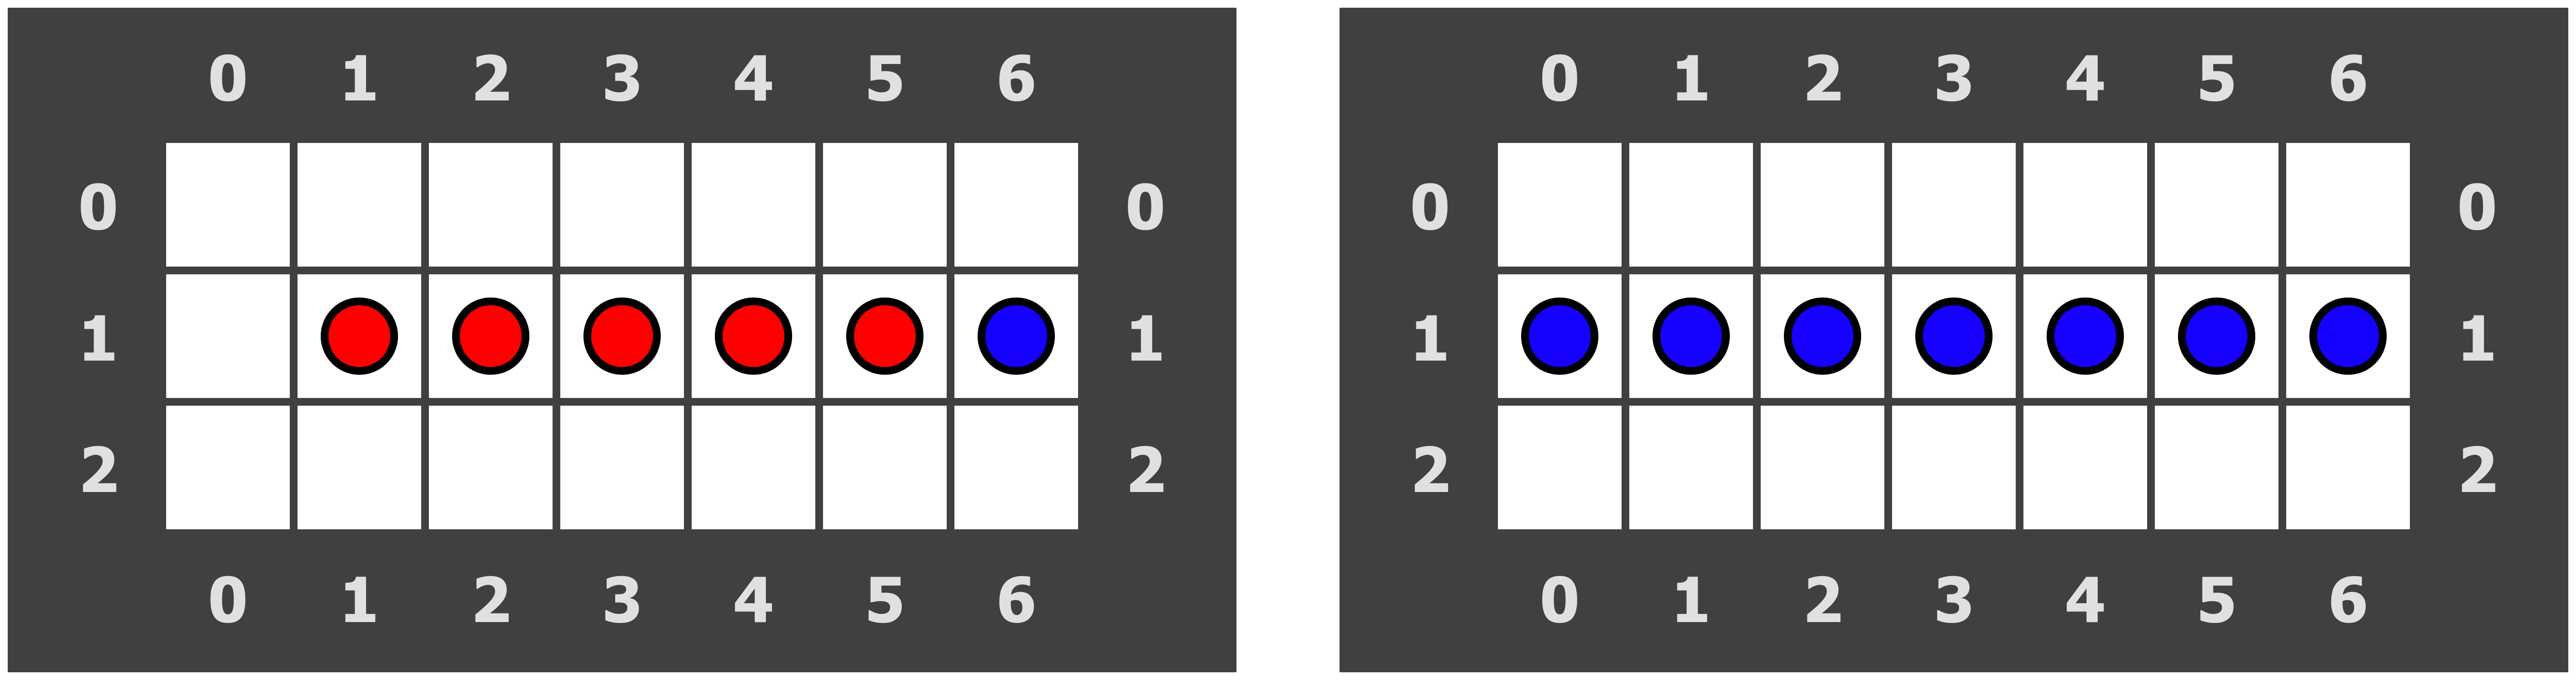
\includegraphics[width=0.6\linewidth]{pics/naive-game-situation}
    \captionof{figure}[Spielfeldsituation 01]{Problematik der naiven Bewertung}
    \label{fig:naivespielfeld01}
\end{minipage}

\subsection{Bestandteile der Heuristik}\label{subsec:bestandteile-der-heuristik}
Wie bereits in der Einleitung gezeigt, gen\"ugt das reine Abz\"ahlen der Spielsteine nicht aus.
Deshalb setzen wir auf drei unterschiedliche Heuristiken, um die aktuelle Spielsituation zu bewerten.
Unter diesen drei Ans\"atzen werden die Mobilit\"at der Spieler, das Verh\"altnis der Spielsteine sowie die aktuelle Bewertung der Karte miteinbezogen.
Diese einzelnen Bestandteile sind w\"ahrend dem Spiel jedoch nicht immer gleichbedeutend, da zum Beispiel im fr\"uhen Spielverlauf die Mobilit\"at und das Besetzen von wichtigen Feldern von Vorteil ist.
Im sp\"ateren Spielverlauf m\"ussen die einzelnen Bestandteile anders gewertet werden.
Hierbei muss darauf geachtet werden, seine Anzahl an Steinen zu erh\"ohen.

\subsubsection{Gewichtung des Spielfeldes}\label{subsubsec:gewichtung-des-spielfeldes}
Es gibt gewisse Positionen die f\"ur einen Spieler wertvoller sind als andere.
Zu diesen Positionen z\"ahlen unter anderem Kanten und Ecken, da es wesentlich schwieriger, bis garnicht m\"oglich ist, diese einzunehmen.
Eine Ausnahme stellt hier das Einnehmen mithilfe von \"Uberschreib-, bzw.\ Spezialsteine dar.
Insbesondere sind Felder die zwei Felder oder mehr von einem Bonusfeld in direkter Richtung entfernt sind h\"oher gewichtet, da sie die M\"oglichkeit geben einen solchen Bonusstein einzunehmen falls ein Gegner auf ein direktes Nachbarfeld des Spezialfeldes zieht.

\vspace{1em}
\begin{minipage}{\linewidth}
    \centering
    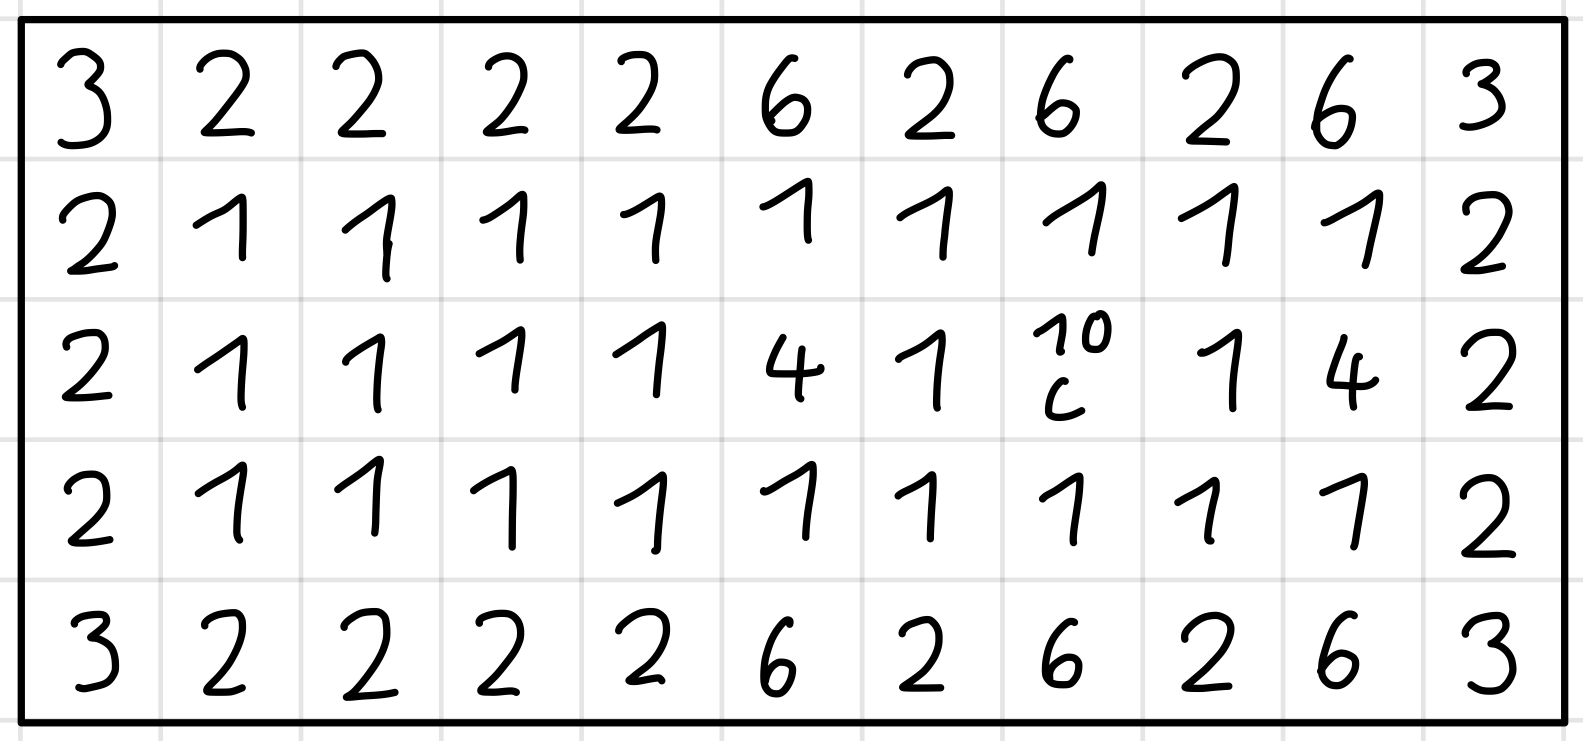
\includegraphics[width=0.5\linewidth]{pics/rating}
    \captionof{figure}[Bewertungsverfahren 01]{Spielfeldpositionen mit Gewichtungen}
    \label{fig:bewertungsverfahren01}
\end{minipage}

Der Score eines Spielers setzt sich dann aus der Summe der belegten Felder mit der entsprechenden Gewichtung zusammen.

Dieses Bewertungsverfahren bietet Vor- und Nachteile.
Positiv daran ist, dass bei Beginn des Spieles jedem Feld eine Gewichtung zugeteilt wird und diese nur noch durch erreichen von Spezialfeldern geringf\"ugig ge\"andert wird.
Negativ ist jedoch, dass dieses Bewertungsverfahren besonders bei gro"sen rechteckigen Spielfeldern mit wenig Spezialfeldern ann\"ahernd wie die naive Variante funktioniert.

\subsubsection{Mobilit\"at}\label{subsubsec:mobilitaet}
Ein weiterer Bestandteil der Analyse besteht darin, Spielsituationen anhand der Beweglichkeit der Spieler einzustufen.
Hierbei wird die Anzahl an Spielz\"ugen eines jeden Spielers bestimmt und miteinander verglichen.
Wie bereits in der Einleitung gezeigt kann ein Spieler seine positive Stellung nur halten, solange er weiterhin spielf\"ahig bleibt.
Aus diesem Grund wird in diesem Ansatz bestimmt wie beweglich ein Spieler gegen\"uber den Anderen ist.

Ein Vorteil dieser Bewertungsmethode besteht darin, dass ein Spieler mit wenig Steinen aber einer hohen Mobilit\"at bei diesem Verfahren nicht negativ bewertet wird.
Ein Problem daran ist jedoch, dass zum Ende des Spieles dieser Ansatz an Relevanz verliert, da zum Schluss nur die Anzahl an eigenen Steinen wichtig ist.

\subsubsection{Spielfeldbelegung}\label{subsubsec:spielfeldbelegung}
Da es besonders gegen Ende des Spiels wichtig ist, viele Steine zu besitzen, muss man dies ebenfalls in die Bewertung miteinbeziehen.
Anstatt aber nur einfach die Anzahl der Spielsteine zu z\"ahlen, wird hier das prozentuale Verh\"altnis gegen\"uber allen existierenden Spielsteinen genommen.

Der Vorteil dieses Verfahrens ist hier, dass man vor allem im sp\"ateren Spielverlauf feststellen kann, wie der aktuelle Stand des Spiels ist und welche Spieler es anzugreifen gilt.
Der Nachteil hierbei ist aber, dass dieses Verfahren im anf\"anglichen und mittleren Spielverlauf nicht aussagekr\"aftig ist.
Allerdings muss man diese Berechnung wie Anfangs erw\"ahnt mit einflie"sen lassen, da man zum Schluss einen Greedyansatz w\"ahlen muss.
Denn letztlich ist f\"ur das Gewinnen des Spieles nur die Anzahl an Spielsteinen von Bedeutung.


\subsection{Algorithmen der Zugauswahl}\label{subsec:algorithmen-der-zugauswahl}
F\"ur einen Computer ist es unm\"oglich den besten Spielzug zu finden, da hier jedes m\"ogliche Spielfeld \"uberpr\"uft werden m\"usste.
Bei einem Spiel wie Schach w\"aren dies circa $10^{120}$ unterschiedliche Spielbrettzust\"ande\footnote{epubli: Zahlen am Brett, \textit{https://www.schachlich.de/schach-in-zahlen/} (abgerufen am 09.05.2021)}.
Bei ReversiXT liegt die Zahl wesentlich h\"oher, da es zum einen viel gr\"o"sere Karten und zum anderen bis zu 8 Spieler gibt.
Damit ein Computer trotzdem einen guten Zug abliefern kann, ben\"otigt es spezielle Algorithmen.
Ein weit verbreiteter Algorithmus f\"ur Zwei-Personen-Nullsummenspiele\footnote{Duden: Spiel, bei dem die Summe der Einsätze, Verluste und Gewinne gleich null ist} lauter Minimax.

\subsubsection{Minimax Algorithmus}\label{subsubsec:minimax-algorithmus}
Zur Veranschaulichung von Minimax soll ein kurzes Gedankenexperiment (siehe Abbildung~\ref{fig:thought-experiment}) dienen, was auch f\"ur fortlaufende Verbesserungen dienen wird.
Es gibt zwei Personen.
Die eine hat zwei Schubl\"aden A \& B mit je zwei Gegenst\"anden.
Die andere Person darf sich nun einen Schubladen aussuchen, aus dem Sie dann ein Geschenk bekommt.
Nun muss sich der Besitzer dieser Gegenst\"ande aussuchen welches er dem Gl\"ucklichen schenken m\"ochte.
Freilich wird er den Gegenstand w\"ahlen, der f\"ur Ihn am wenigsten Verlust darstellt.
Aus diesen Grund macht es keinen Sinn die Schublade B auszuw\"ahlen, da man hier den Gegenstand f\"ur 1~\euro{} bekommt, andernfalls den f\"ur 20~\euro{}.

\vspace{1em}
\begin{center}
    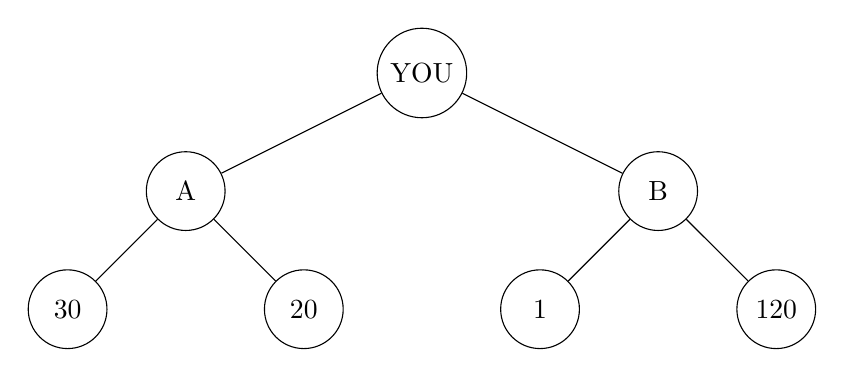
\begin{tikzpicture}[
        level distance=15mm,
        every node/.style={circle,draw,minimum size=1cm},
        level/.style={sibling distance=60mm/#1}
    ]

        \node{\avlkey{YOU}}
            child {node {\avlkey{A}}
                child {node {\avlkey{30}}}
                child {node {\avlkey{20}}}
            }
            child {node {\avlkey{B}}
                child {node {\avlkey{1}}}
                child {node {\avlkey{120}}}
            }
        ;
    \end{tikzpicture}
    \captionof{figure}[Gedankenexperiment]{Grafik zur Veranschaulichung des Gedankenexperimentes.}
    \label{fig:thought-experiment}
\end{center}

Ein solches Verfahren kann nun genutzt werden um unterschiedliche Spielz\"uge gegeneinander zu vergleichen und den Bestm\"oglichen - unter Ber\"ucksichtung der sp\"ateren Z\"uge des Gegners - auszuw\"ahlen.
Jedoch beinhaltet dieser Algorithmus einen Nachteil - es werden auch Spielz\"uge betrachtet die garnicht in Frage kommen, da ein Spieler diesen Zug niemals w\"ahlen w\"urde.

\subsubsection{Alpha-Beta-Pruning}\label{subsubsec:alpha-beta-pruning}
Dieses Problem kann mithilfe dem Alpha-Beta-Pruning drastisch reduziert werden.
Hierbei werden Hilfsvariablen (alpha und beta) durchgereicht.
Mithilfe dieser Verbesserung werden Zugfolgen, die das Ergebnis nicht beeinflussen, erst garnicht kontrolliert.
Beim Gedankenexperiment muss somit nach dem Gegenstand mit Kosten 1~\euro{} keine weiteren Knoten angeschaut werden, da der Spieler YOU diesen Pfad (im Beispiel die Schublade B) nicht w\"ahlen wird.
Das liegt daran, dass f\"ur ihn die Schublade A wesentlich interessanter ist.
Selbstverst\"andlich nur unter Ber\"ucksichtigung, dass der Andere seinen Verlust minimieren m\"ochte.

\subsubsection{Vergleich der Algorithmen}\label{subsubsec:vergleich-der-algorithmen}
Um die Bedeutung dieser Variante zu verdeutlichen folgt nun ein Vergleich beider Verfahren.
Dabei wurden die selbe Karte mit unterschiedliche Suchbaumtiefen getestet.
Es trat in den Tiefen 3 bis 8 jeweils zwei Spieler gegeneinander an\footnote{Die Suchbaumtiefe 8 wurde auf einem Labor-PC der OTH Regensburg durchgef\"uhrt. N\"ahere Informationen siehe Kapitel~\ref{subsec:technische-daten}}.
Es wurde je einmal der erste Spieler und einmal der zweite Spieler mit Alpha-Beta gestartet.

\vspace{1em}
\begin{minipage}{\linewidth}
    \centering
    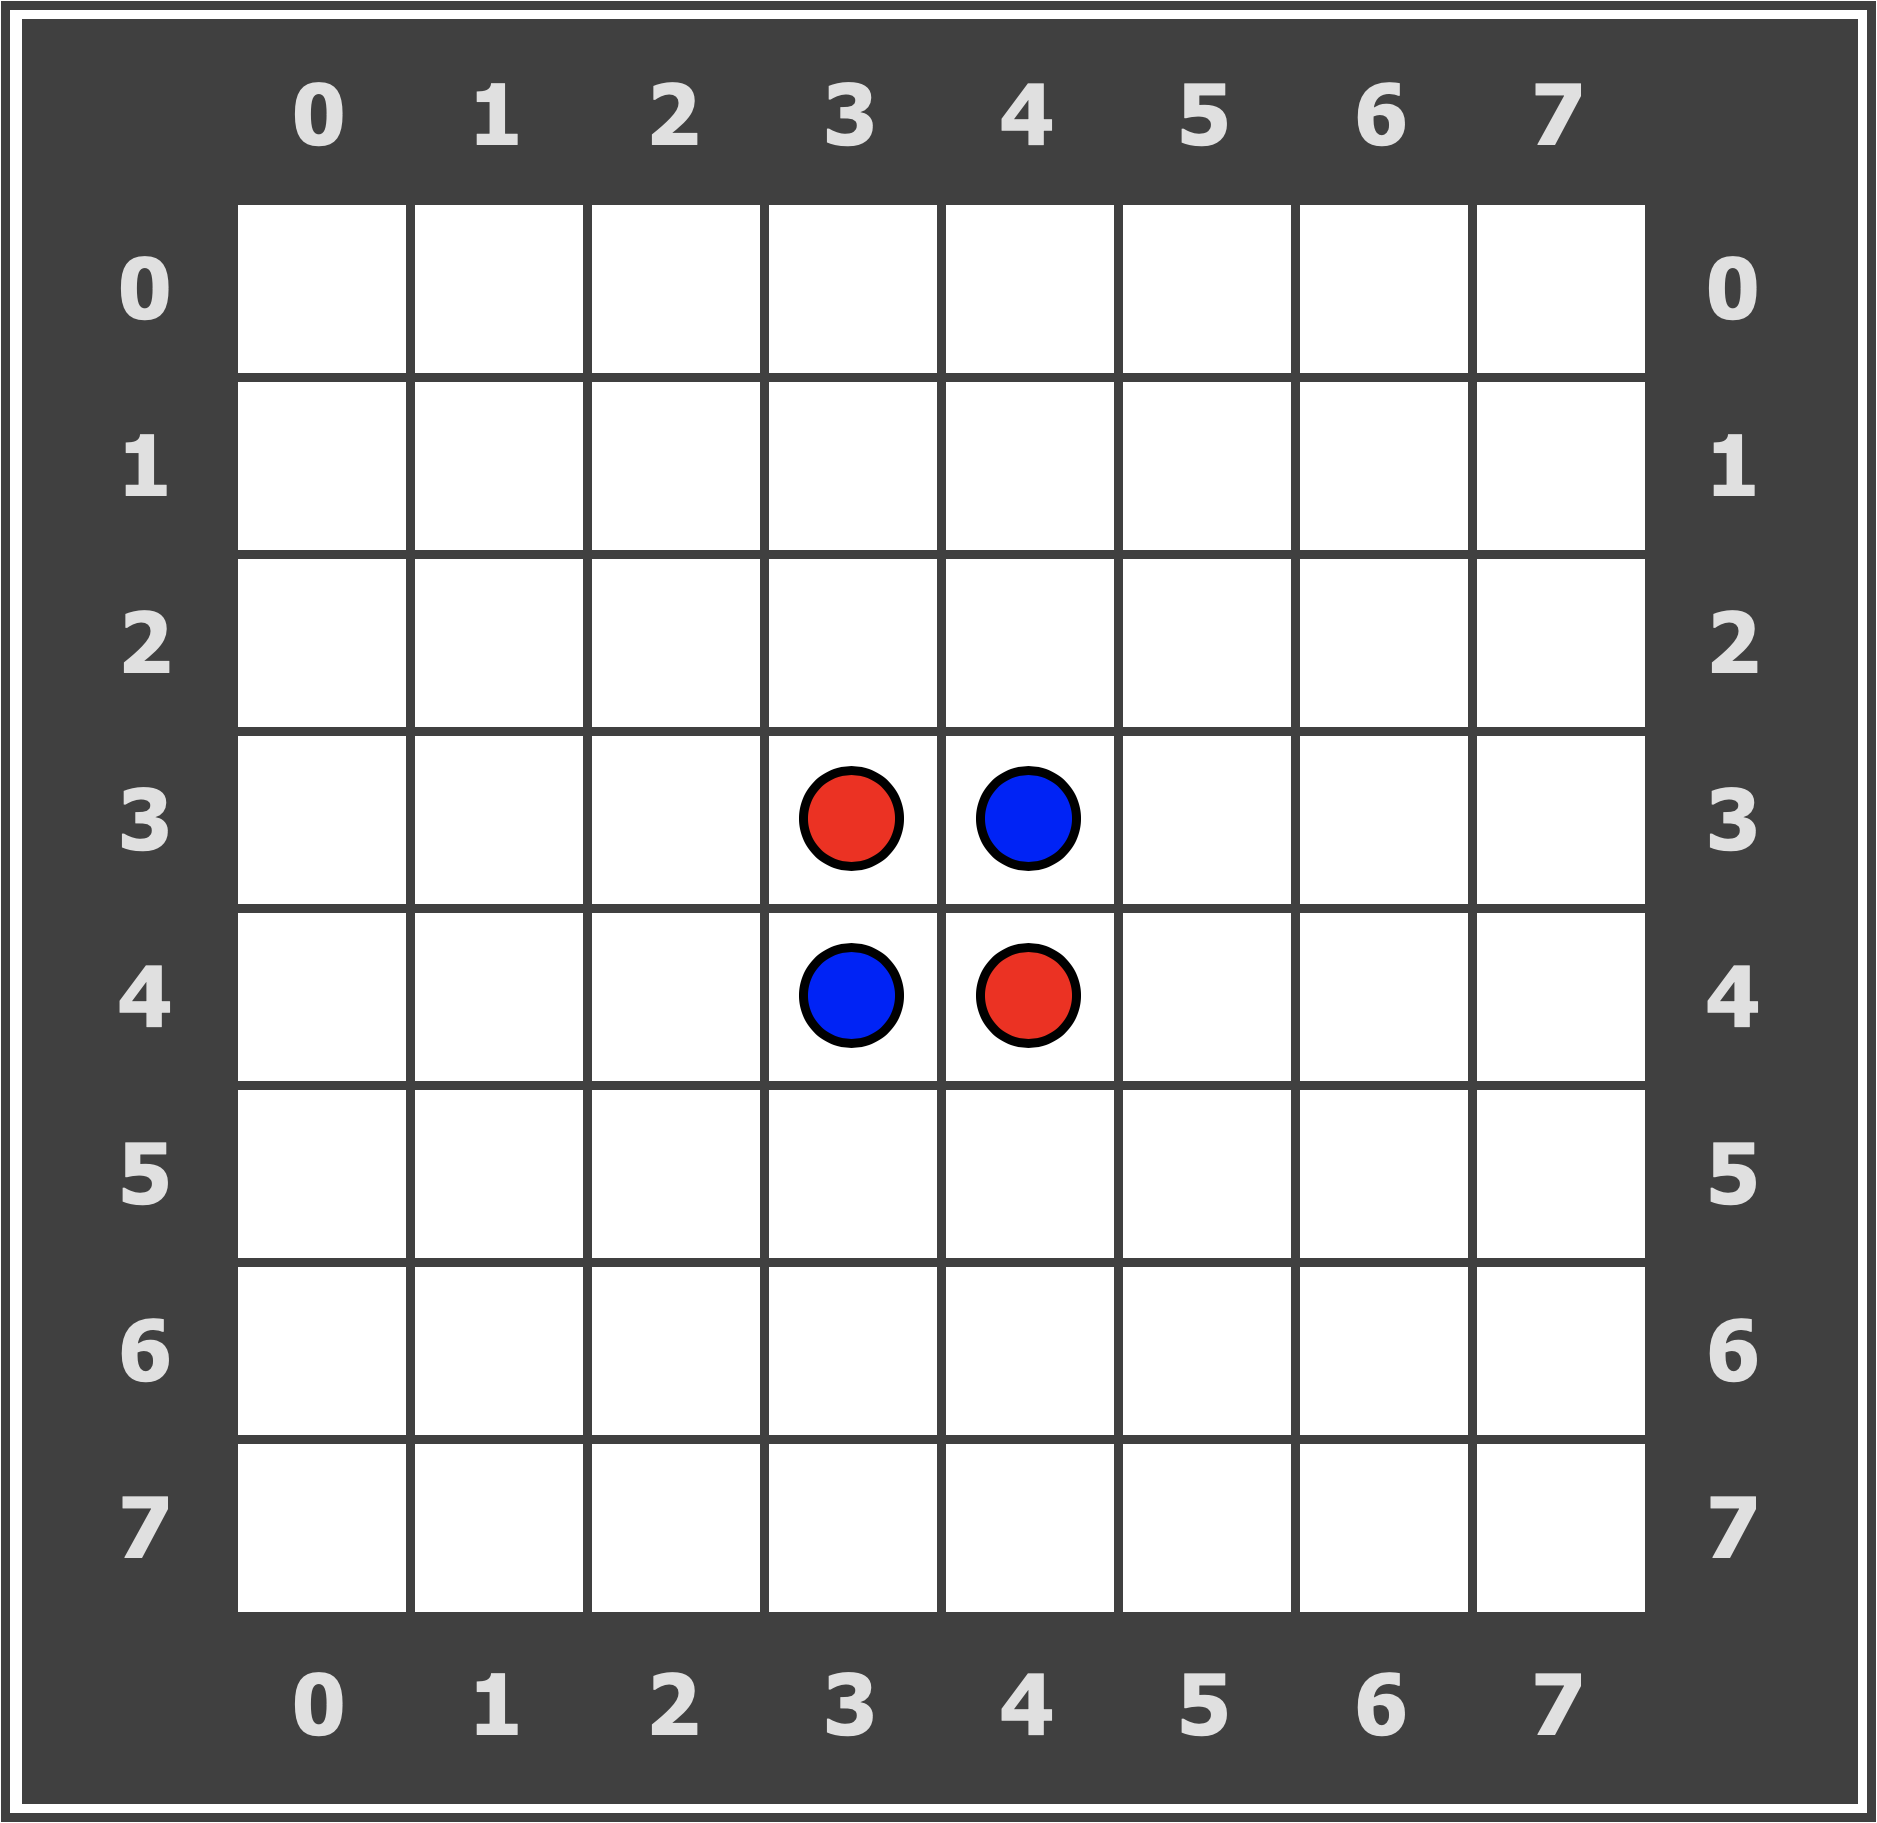
\includegraphics[width=0.3\linewidth]{pics/statistic-map}
    \captionof{figure}[Karte für Statisitk]{Verwendete Karte für den Vergleich von Minimax und Alpha-Beta}
    \label{fig:statistic-map}
\end{minipage}

Wir haben uns aus folgenden Gr\"unden f\"ur die Karte aus Abbildung~\ref{fig:statistic-map} entschieden:
\begin{enumerate}
    \item Es gibt nur zwei Spieler, womit beide Verfahren gegeneinander antreten k\"onnen.
    \item Es gibt keine Spezialsteine, was das Spiel einfacher gestaltet und beim Vergleich der Algorithmen nicht von Bedeutung ist.
    \item Die verwendete Karte ist komplett symmetrisch, wodurch eine Fairness f\"ur beide Spieler garantiert wird.
    \item Es handelt sich um eine relativ kleine Karte, damit die Berechnungen zeitlich einigerma"sen eingegrenzt werden k\"onnen.
\end{enumerate}

\vspace{1em}
\begin{minipage}{\linewidth}
    \centering
    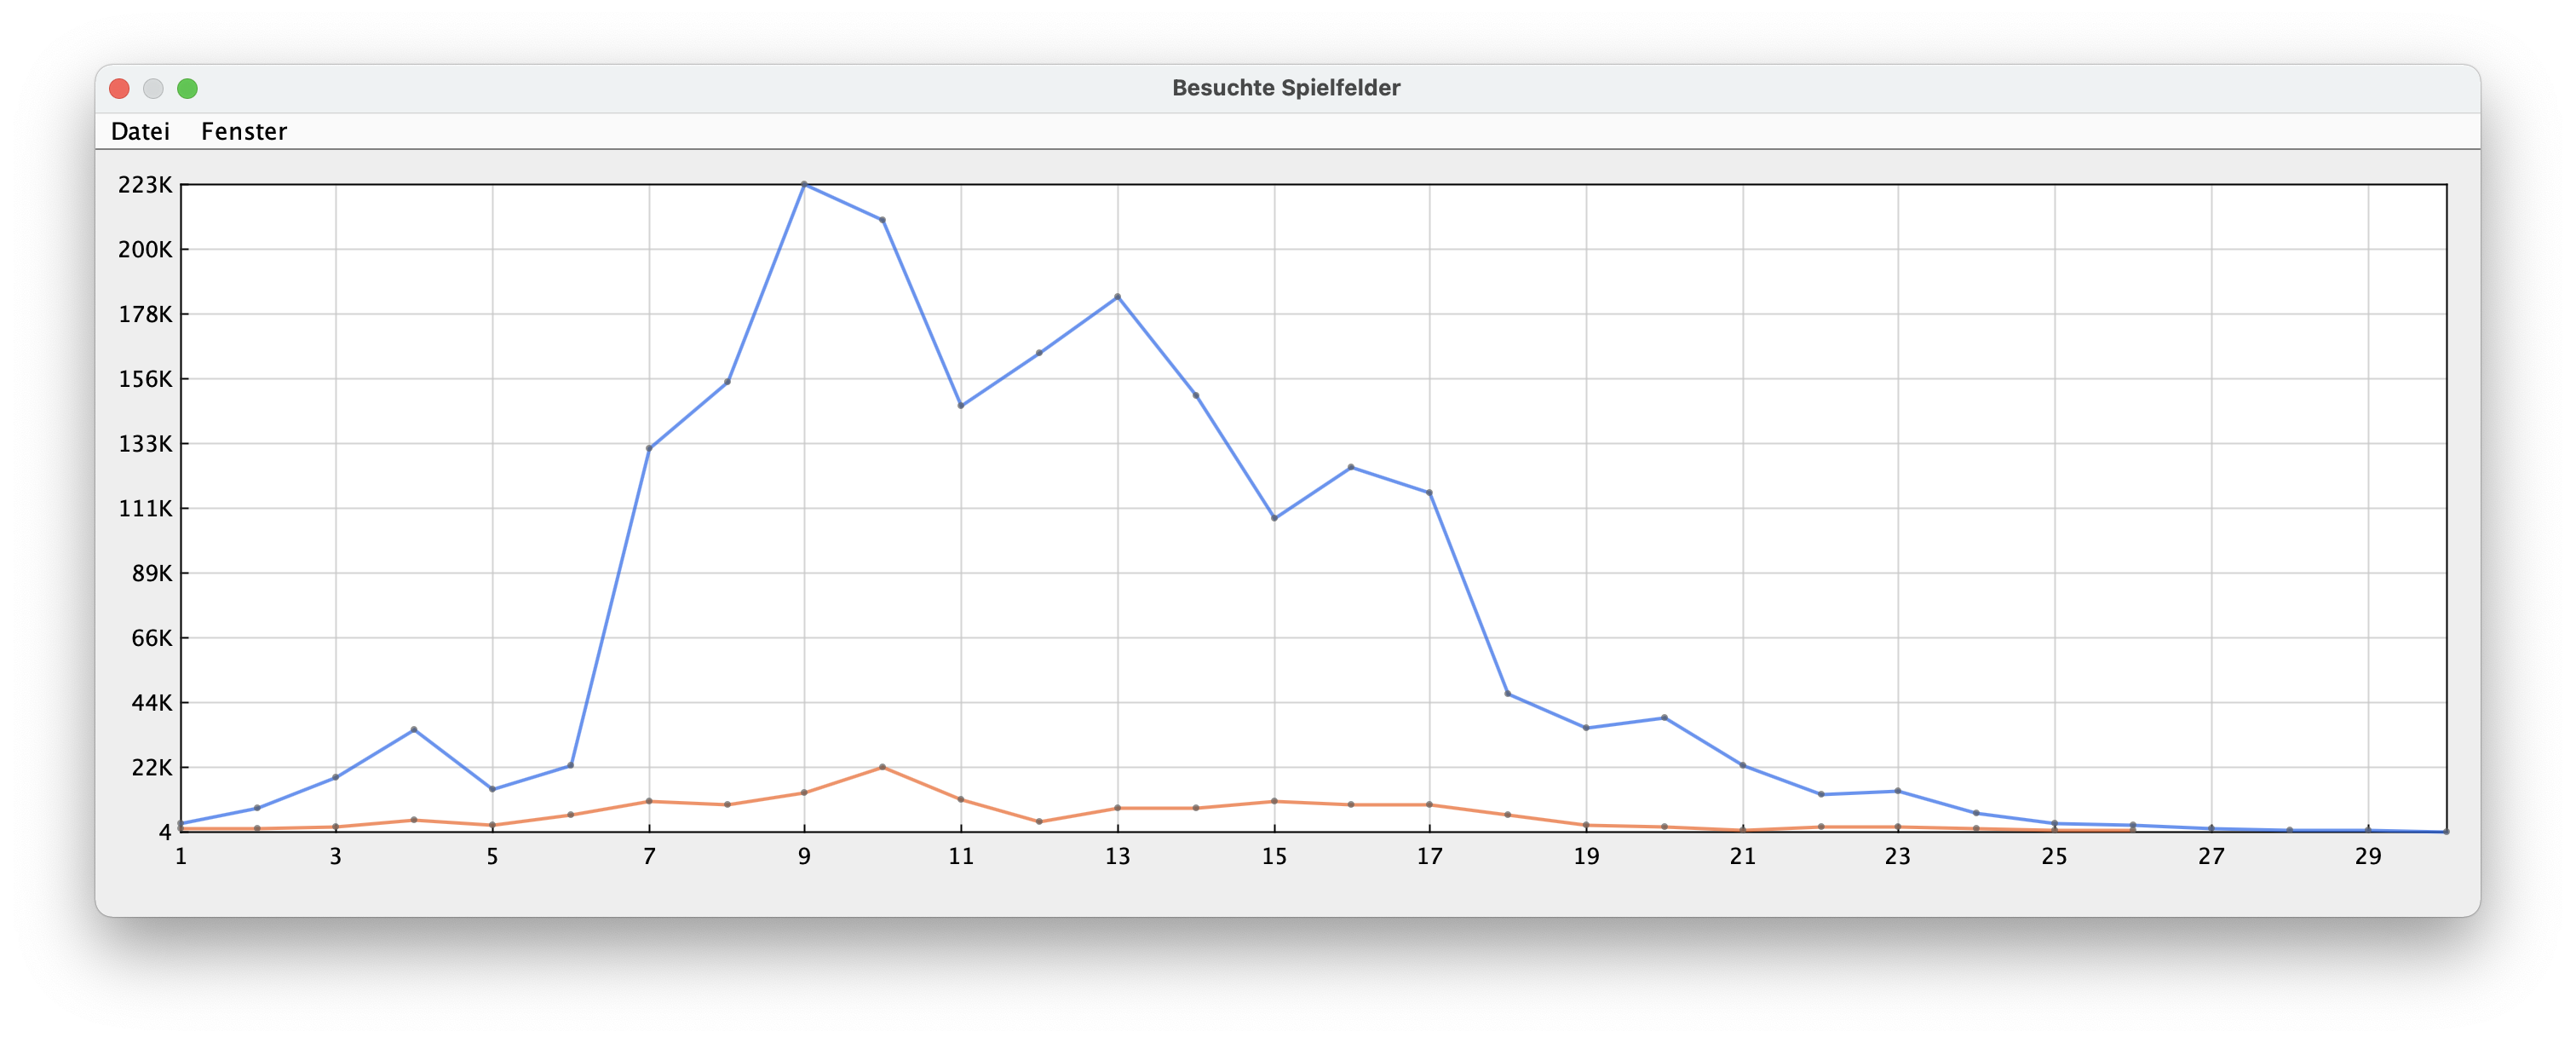
\includegraphics[width=0.9\linewidth]{statistic/Test-D5-01/ST-01-D5-LD}
    \captionof{figure}[Statistik für Tiefe 5]{Diese Statistik wurde bei einem Spiel der Tiefe 5 aufgenommen.}
    \label{fig:statistic-screen}
\end{minipage}

In Abbildung~\ref{fig:statistic-screen} sind sowohl \"uberpr\"ufte Karten ohne Alpha-Beta (blaue Linie), als auch mit Alpha-Beta (orange Linie) zu sehen.
Hierbei ist klar ersichtlich, das Alpha-Beta-Pruning einen enormen Leistungsvorteil liefert.
Der obige Screenshot stammt aus der selbstentwickelten Software GameAnalyzer.
Mehr dazu in Kapitel~\ref{sec:spielanalyse}.

Die Tabelle~\ref{tab:search-depth} liefert eine \"Ubersicht \"uber alle getesteten Suchbaumtiefen dieser Karte.

\vspace{1em}
\begin{table}[!h]
    \centering
    \begin{tabular}{|l|c|c|}
        \hline
        \textbf{Tiefe} & \textbf{Alpha-Beta} & \textbf{Minimax}\\
        \hline
        3 & 1.079,5 & 2.434,5\\
        \hline
        4 & 5.985,5 & 18.417,5\\
        \hline
        5 & 22.653 & 244.854,5\\
        \hline
        6 & 133.657,5 & 1.313.347\\
        \hline
        7 & 419.537 & 28.802.230\\
        \hline
        8 & ? & ?\\
        \hline
    \end{tabular}
    \caption{Besuchte Karten mit den Suchalgorithmen. (Ergebnisse wurden geglättet)}
    \label{tab:search-depth}
\end{table}

Auf den ersten Blick wirken diese Zahlen nun ziemlich bedeutungslos.
Werden Sie jedoch in ein Koordinatensystem (siehe Abbildung~\ref{fig:statistic-graph}) eingetragen und eine Linie eingezeichnet, kann man den Verlauf bei weiteren Suchbaumtiefen beider Algorithmen erahnen.

\vspace{1em}
\begin{minipage}{\linewidth}
    \centering
    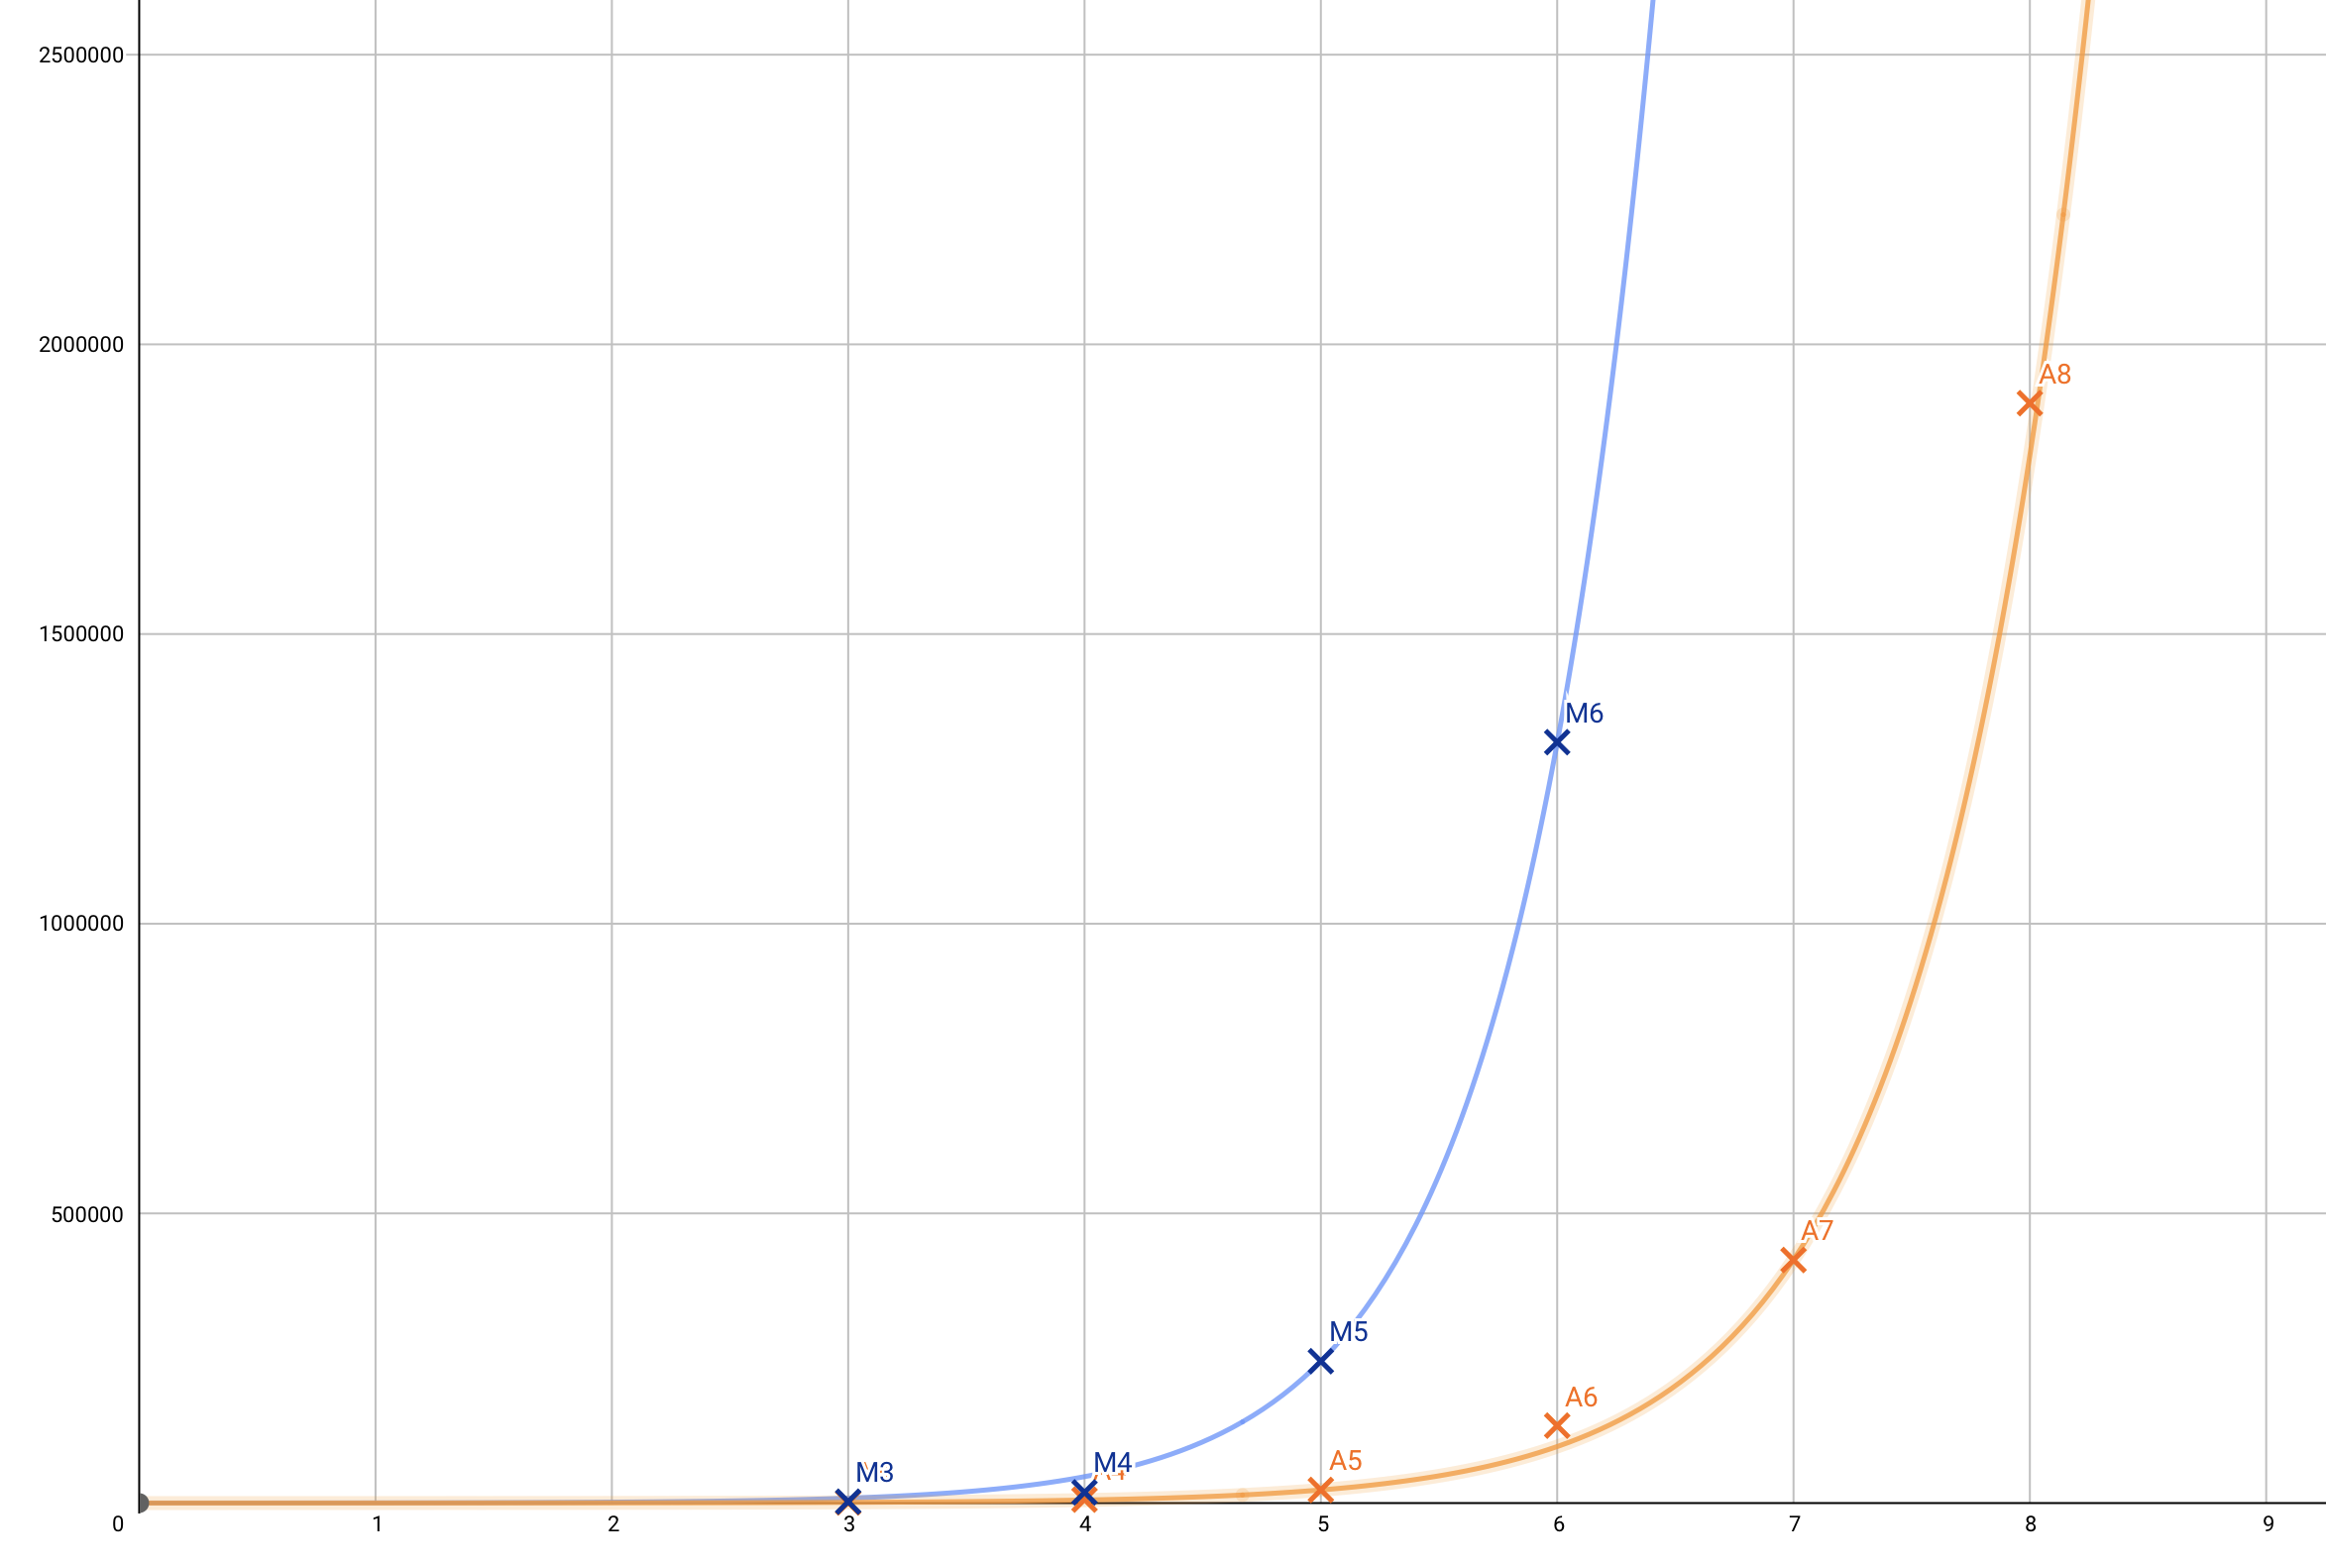
\includegraphics[width=0.7\linewidth]{pics/statistic-graph}
    \captionof{figure}[Suchbaumtiefen in Koordinaten]{Suchbaumtiefen in ein Koordinatensystem eingetragen.}
    \label{fig:statistic-graph}
\end{minipage}

Der Aufwand aller m\"ogliche Spielzust\"ande zu vergleichen w\"achst bei beiden Verfahren exponentiell mit der Anzahl der Suchbaumtiefe.
Jedoch bewirkt des Alpha-Beta-Pruning eine gestauchtere Kurve als der Minimax-Algorithmus ohne Alpha-Beta-Pruning.

Bei gleicher Anzahl an analysierten Felder kann somit mit Alpha-Beta-Pruning weiter in den Suchbaum hineingeschaut und dadurch mehr Z\"uge miteinander verglichen werden.
Das f\"uhrt dazu, dass bei gleichem Zeitaufwand (= gleiche Anzahl an analysierten Spielzust\"anden), das beste Ergebnis einer tieferen Suchbaumebene gefunden wird.

\bigskip
\newpage